\chapter{Reformulación del Control como un problema de inferencia}%
\label{cha:reformulación_del_control_como_un_problema_de_inferencia}

\lecture{14}{2020-07-04}{Reframing Control as an Inference Problem}

\section{¿El control óptimo y RL son capaces de proveer un modelado razonable del
comportamiento humano?}%
\label{sec:_el_control_óptimo_y_rl_son_capaces_de_proveer_un_modelado_razonable_del_comportamiento_humano_}

Este tema será un poco más teórico y el siguiente más práctico.

\subsection{Control Óptimo como un modelo del comportamiento humano}%
\label{sub:control_óptimo_como_un_modelo_del_comportamiento_humano}

Desde hace mucho tiempo (Muybridge, 1870) se ha intentado explicar el comportamiento
humano como una búsqueda de la optimalidad de una tarea, como por ejemplo correr minimizando
la energía utilizada. Hoy en día se puede modelar bastante bien (clase de hoy) y también hay
ejemplos del modelado probabilístico de conductores de taxi.

La idea es la siguiente: si se tiene una función de recompensa y una forma de modelar el mundo
o interactuar con él se puede extraer una planificación óptima resolviendo un problema de
optimización.

Pero el comportamiento de las personas y animales es más complejo. Por ejemplo si se tiene
a un mono y se le pide que lleve un punto en la pantalla hasta otro que es el destino mediante
un joystick, no hará una trayectoria en línea recta perfecta, que sería lo más óptimo. En su
lugar haría una trayectoria parecida pero curva, ya que es lo más fácil de hacer llegando aún
así al destino. Incluso las trayectorias se verán influenciadas por el día y su estado de ánimo.
En resumen, su comportamiento es estocástico, pero las buenas acciones son las más probables.

Teniendo esto en cuenta, hay que tirar a la basura los objetivos que se tenían antes:
\begin{align}
    a _ { 1 } , \ldots , a _ { T } &= \operatorname { arg } \operatorname { max } _ { a _ { 1 } ,
\ldots , a _ { T } } \sum _ { t = 1 } ^ { T } r ( s _ { t } , a _ { t } )\\
        s _ { t + 1 } &= f ( s _ { t } , a _ { t } )
\end{align}
ya que únicamente dan como óptimo la línea recta. Para explicar las acciones aleatorias del mono,
se necesita un modelo gráfico:
\begin{figure}[H]
	\centering
	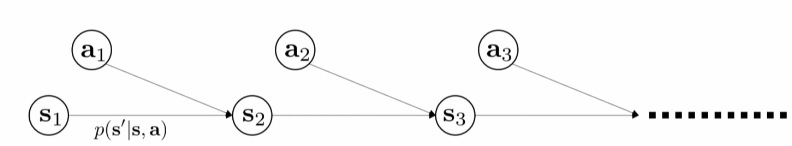
\includegraphics[width=0.8\linewidth]{figures/2020-07-04-175014_792x146_scrot.png}
\end{figure}
Se puede escribir la probabilidad de ver una secuencia de estados con otra secuencia de
acciones:
\begin{align}
    p ( s _ { 1 : T } , a _ { 1 : T } ) = ?? \text{ no existe ninguna asunción de
    comportamiento óptimo }
\end{align}
El modelo que se tiene no dice que los pares de acciones-estados sean óptimos, simplemente
si son físicamente posibles. Por lo que se le añade al grafo los nodos $O$ (por optimalidad)
para cada paso en el tiempo. Lo que representan estas variables es si se está siendo óptimo o
no, por lo que es una variable binaria. También se puede pensar en esta variable como la
intencionalidad.
\begin{figure}[H]
	\centering
	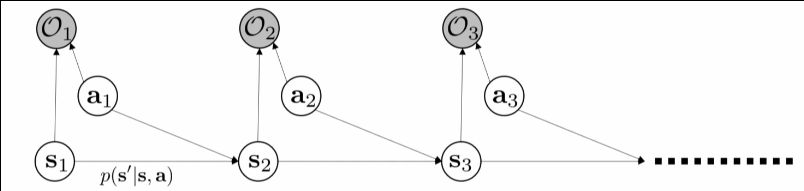
\includegraphics[width=0.8\linewidth]{figures/2020-07-04-175416_804x191_scrot.png}
\end{figure}
Para modelar el comportamiento del mono, se introduce lo siguiente:
\begin{align}
    \label{eq:mono}
    p(\tau|O_{1:T}) \quad\quad p(O_t|s_t,a_t)=\exp( r(s_t,a_t) )
\end{align}
El término de la izquierda significa cuál es la probabilidad de la trayectoria $\tau$
si nuestro mono siempre se comporta de forma óptima. Para el de la derecha, se elige arbitrariamente la
probabilidad del comportamiento óptimo para ese paso en el tiempo como la exponencial de la
recompensa si se toma la acción $a_t$. Si se quiere normalizar se puede restar por la
exponencial de la recompensa más grande. Esta elección arbitraria tendrá sentido más
adelante. Con lo que se tiene en \ref{eq:mono}, se deriva:
\begin{align}
    p ( \tau | O _ { 1 : T } ) &= \frac { p ( \tau , O _ { 1 : T } ) } { p ( O _ { 1 : T } ) }\\
    \propto p ( \tau ) \prod _ { t } \operatorname { exp } \left( r ( s _ { t } , a _ { t } )
\right) &= p ( \tau ) \operatorname { exp } \left( \sum _ { t } r ( s _ { t } , a _ { t } )
\right)
\end{align}

 Esto es interesante porque puede modelar comportamientos subóptimos, lo cual es importante
 para RL inverso. También se puede aplicar para resolver problemas de control y
 planificación. Además da una explicación de porque un comportamiento estocástico puede
 ser más preferible que uno determinista (útil para la exploración y \textit{transfer
 learning}).

 \subsection{Inferencia en este modelo}%
 \label{sub:inferencia_en_este_modelo}
 
 El modelo gráfico anterior tiene dos tipos de distribuciones condicionales:
 \begin{itemize}
     \item Dinámicas: $p(s_{t+1}|s_t,a_t)$ 
     \item Exponencial de la recompensa: $p(O_t|s_t,a_t)\propto \exp(r(s_t,a_t))$
 \end{itemize}
 Además para el primer estado se tiene $p(s_1)$.

 Para realizar la inferencia, se hacen tres preguntas:
 \begin{enumerate}
     \item ¿Como se calcula un mensaje hacia atrás?\\Un mensaje hacia atrás se define como
         $\beta_t(s_t,a_t)=p(O_{t:T}|s_t,a_t)$ y es la probabilidad de que las variables de
         optimalidad $O$ desde el tiempo actual $t$ hasta el final $T$ sean verdaderas dado
         $(s_t,a_t)$. Parece una pregunta un tanto arbitraria pero con esto se pude recuperar
         una política casi óptima en este modelo.
     \item ¿Cómo se calcula la política $p(a_t|s_t,O_{1:T})$? Esta distribución
         condicional es equivalente a la política óptima bajo este modelo gráfico. Resuelve la
         pregunta de: dado el estado actual y dado a que todas futuras acciones sean
         tomadas óptimamente, cuál es la probabilidad de tomar la acción $a_t$.\\Resolver la
         pregunta 1 ayuda a resolver la pregunta 2.
     \item ¿Cómo se calcula un mensaje hacia adelante
         $\alpha_t(s_t)=p(s_t|O_{1:t-1})$? Un mensaje hacia adelante te da la probabilidad de
         acabar en el estado $s_t$ sabiendo que se ha tenido un comportamiento
         óptimo en todos los estados anteriores. No se necesita para calcular la
         política. Pero es muy útil para saber en que estados la política óptima cae. Son
         necesarios para resolver RL inverso.
 \end{enumerate}

 \subsubsection{Mensajes hacia atrás}%
 \label{ssub:mensajes_hacia_atrás}
 
De los tres anteriores son los más útiles.

Como se dijo, se definen como:
\begin{align}
\beta _ { t } ( s _ { t } , a _ { t } ) = p ( O _ { t : T } | s _ { t } , a _ { t } )
\end{align}
Se va a expresar $\beta$ en función de la probabilidad de transición y la probabilidad de la
optimalidad, y como esto es un proceso iterativo, también en $\beta_{t+1}$.
\begin{align}
    \beta_t(s_t,a_t)&=\int p ( O _ { t : T } , s _ { t + 1 } | s _ { t } , a _ { t } ) d s _ { t
    + 1 }\\
    & = \int p ( O _ { t + 1 : T } | s _ { t + 1 } ) p ( s _ { t + 1 } | s _ { t } , a _ { t } ) p ( O _ { t } | s _ { t } , a _ { t } ) d s _ { t + 1 }
\end{align}
El paso de 12.8 a 12.9 se puede hacer aplicando la regla de la cadena de la probabilidad porque $O_t$ es independiente de $O_{t+1}$ dado $s_{t+1}$.
De 12.9, se conoce $p(O_t|s_t,a_t)$ (la recompensa), $p(s_{t+1}|s_t,a_t)$ también se conoce
por lo que nos quedamos solo con $p(O_{t+1:T}|s_{t+1})$. A este término se le 'inserta la
acción':
\begin{align}
p ( O _ { t + 1 : T } | s _ { t + 1 } ) = \int p ( O _ { t + 1 : T } | s _ { t + 1 } , a _ { t + 1 } ) p ( a _ { t + 1 } | s _ { t + 1 } ) d a _ { t + 1 }
\end{align}
El primer término del producto es igual a $\beta_t{s_{t+1},a_{t+1}}$. El segundo,
$p(a_{t+1}|s_{t+1})$ nos dice que probabilidad tenemos de poder tomar cualquier acción
sobre el estado $s_{t+1}$. Como prácticamente se pueden tomar todas las acciones que sean
físicamente posibles, se puede simplificar como una distribución uniforme. Esta asunción no
reduce la generalidad de esta formulación.

Por ahora se está asumiendo que se conocen todas las probabilidades (modelo, \ldots), en la
práctica se tendrán que tomar muestras.

\begin{algorithm}
    \caption{Paso hacia atrás}
    \For{$t=T-1$ hasta  $1$}{
        $ \beta _ { t } ( s _ { t } , a _ { t } ) = p ( O _ { t } | s _ { t } , a _ { t } ) E _ {
        s _ { t + 1 } \sim p ( s _ { t + 1 } | s _ { t } , a _ { t } ) } [ \beta _ { t + 1 } ( s
        _ { t + 1 } ) ] $\\
        $ \beta _ { t } ( s _ { t } ) = E _ { a _ { t } \sim p ( a _ { t } | s _ { t } ) } [
        \beta _ { t } ( s _ { t } , a _ { t } ) ]$
    }
\end{algorithm}

Se puede pensar que el segundo paso tiene un aspecto familiar. Se introducen las siguientes variables
arbitrariamente.
\begin{align}
\left. \begin{array} { l } { V _ { t } ( s _ { t } ) = \operatorname { log } \beta _ { t } ( s _ { t } ) } \\ { Q _ { t } ( s _ { t } , a _ { t } ) = \operatorname { log } \beta _ { t } ( s _ { t } , a _ { t } ) } \end{array} \right.
\end{align}
Que son básicamente los mensajes hacia atrás en espacio logarítmico. Expandiendo con la
definición, se tiene que:
\begin{align}
V _ { t } ( s _ { t } ) = \operatorname { log } \int \operatorname { exp } ( Q _ { t } ( s _ { t } , a _ { t } ) ) d a _ { t }
\end{align}
Si se tienen valores de $Q$ muy grandes para una cierta acción, este silenciará a los
valores más pequeños ya que las diferencias debido a la exponencial serán muy grandes. Este
efecto se ve aún más acentuado después de aplicar el logaritmo. Por lo que según $Q_t(s_t,a_t)$
se va haciendo más grande, $V_t(s_t)\rightarrow \max_{a_t}Q_t(s_t,a_t)$. Esto será de utilidad
más adelante.

Para el primer paso, al expresarlo en el espacio logarítmico:
\begin{align}
Q _ { t } ( s _ { t } , a _ { t } ) = r ( s _ { t } , a _ { t } ) + \operatorname { log } E [ \operatorname { exp } ( V _ { t + 1 } ( s _ { t + 1 } ) ) ]
\end{align}
Como se ha comentado antes, $V_{t+1}$ tenderá a ser $\max_{a_t}Q_{t+1}(s_t,a_t)$ según
$Q_{t+1}$ vaya creciendo. Junto a esto, si se quitan el logaritmo y la exponencial, el paso
es el mismo que el primer paso que en el algoritmo de iteración del valor, donde:
\begin{align}
Q ( s , a ) \leftarrow r ( s , a ) + \gamma E [ V ( s ^ { \prime } ) ]
\end{align}
Con dinámicas deterministas, el logaritmo y la exponencial se cancelan y efectivamente
coincide con este paso.

Para el caso estocástico, esta formulación es un problema porque describe un comportamiento que
no se quiere ver en control óptimo. Esto es porque la transición se convierte en
optimista, lo cual no es una buena idea.

Antes se comentó que como simplificación se puede tener que $p(a_{t+1}|s_{t+1})$ fuera uniforme.
En el caso de que no se quiera que sea uniforme:
\begin{align}
    V ( s _ { t } ) &= \operatorname { log } \int \operatorname { exp } ( Q ( s _ { t } , a _ { t } )
+ \operatorname { log } p ( a _ { t } | s _ { t } ) ) a _ { t }\\
    Q ( s _ { t } , a _ { t } ) &= r ( s _ { t } , a _ { t } ) + \operatorname { log } E [
\operatorname { exp } ( V ( s _ { t + 1 } ) ) ]\\
    \tilde { Q } ( s _ { t } , a _ { t } ) &= r ( s _ { t } , a _ { t } ) + \operatorname { log } p (
a _ { t } | s _ { t } ) + \operatorname { log } E [ \operatorname { exp } ( V ( s _ { t + 1 } ) )
]\\
V ( s _ { t } ) = \operatorname { log } \int \operatorname { exp } ( \tilde { Q } ( s _ { t } , a
    _ { t } ) ) a _ { t } \quad &\Leftrightarrow \quad V ( s _ { t } ) = \operatorname { log } \int \operatorname { exp } ( Q ( s _ { t } , a _ { t } ) + \operatorname { log } p ( a _ { t } | s _ { t } ) ) a _ { t }
\end{align}
Por lo que no cambia mucho la formulación.

\subsubsection{Calcular la política}%
\label{ssub:calcular_la_política}

Se corresponde con la pregunta 'de verdad', ¿cómo calcular la política óptima a partir de
este modelo gráfico $p(a_t|s_t,O_{1:T})$?

Lo que se quiere buscar esencialmente es la política:
\begin{align}
    p(a_t|s_t,O_{1:T})&=\pi(a_t|s_t)\\
                      &=p(a_t|s_t,O_{t:T})\\
                      &= \frac{p(a_t,s_t|O_{t:T})}{p(s_t|O_{t:T})} \\
                      &= \frac { p ( O _ { t : T } | a _ { t } , s _ { t } ) p ( a _ { t } , s _
                      { t } ) / p ( O _ { t : T } ) } { p ( O _ { t : T } | s _ { t } ) p ( s _ {
                  t } ) / p ( O _ { t : T } ) }\\
                      &= \frac { p ( O _ { t : T } | a _ { t } , s _ { t } ) } { p ( O _ { t : T
                      } | s _ { t } ) } \frac { p ( a _ { t } , s _ { t } ) } { p ( s _ { t } ) }
                      =  \frac { p ( O _ { t : T } | a _ { t } , s _ { t } ) } { p ( O _ { t : T
                      } | s _ { t } ) } p(a_t|s_t)\\
                      &= \frac{\beta_t(s_t,a_t)}{\beta_t(s_t)} p(a_t|s_t)
\end{align}
Como $p(a_t|s_t)$ se considera como uniforme, se puede expresar:
\begin{align}
    \pi(a_t|s_t) = \frac{\beta_t(s_t,a_t)}{\beta_t(s_t)}
\end{align}
Sustituyendo $\beta$ por las variables $V$ y $Q$ se obtiene:
\begin{align}
\pi ( a _ { t } | s _ { t } ) = \operatorname { exp } ( Q _ { t } ( s _ { t } , a _ { t } ) - V _ { t } ( s _ { t } ) ) = \operatorname { exp } ( A _ { t } ( s _ { t } , a _ { t } ) )
\end{align}
Por lo que la política es simplemente la exponencial del \textit{advantage}. También se puede
expresar con temperatura de la siguiente forma:
\begin{align}
\pi ( a _ { t } | s _ { t } ) = \operatorname { exp } ( \frac { 1 } { \alpha } Q _ { t } ( s _ { t } , a _ { t } ) - \frac { 1 } { \alpha } V _ { t } ( s _ { t } ) ) = \operatorname { exp } ( \frac { 1 } { \alpha } A _ { t } ( s _ { t } , a _ { t } ) )
\end{align}
Lo que permite convertir la política en estocástica con $\alpha=1$ o determinista
$\alpha=0$.

Como resumen:
 \begin{itemize}
    \item La interpretación natural es que las acciones mejores son las más probables.
    \item Si dos acciones son igual de buenas tendrán la misma probabilidad.
    \item Análogo a la exploración de Boltzmann.
    \item Se aproxima a la política voraz según va decreciendo la temperatura.
\end{itemize}

\subsubsection{Mensajes hacia adelante}%
\label{ssub:mensajes_hacia_adelante}

Los mensajes hacia adelante es la probabilidad de acabar en un estado dado que se hayan
realizado acciones óptimas hasta ese momento, se va a realizar un procedimiento de
expansión parecido al anterior:
\begin{align}
    \alpha _ { t } ( s _ { t } ) &= p ( s _ { t } | O _ { 1 : t - 1 } )\\
                                 &= \int p ( s _ { t } , s _ { t - 1 } , a _ { t - 1 } | O _ { 1
                                 : t - 1 } ) d s _ { t - 1 } d a _ { t - 1 } = \int p ( s _ { t }
                                 | s _ { t - 1 } , a _ { t - 1 } , O _ { 1 \cdot t - 1 } ) p ( a
                                 _ { t - 1 } | s _ { t - 1 } , O _ { 1 : t - 1 } ) p ( s _ { t -
                                 1 } | O _ { 1 : t - 1 } ) d s _ { t - 1 } d a _ { t - 1 }\\
&= \int p ( s _ { t } | s _ { t - 1 } , a _ { t - 1 } ) p ( a _ { t - 1 } | s _ { t - 1 } , O _ { t - 1 } ) p ( s _ { t - 1 } | O _ { 1 : t - 1 } ) d s _ { t - 1 } d a _ { t - 1 }
\end{align}
De los tres términos de 12.30, se conoce el primero que son las dinámicas pero los otros dos
tenemos que trabajarlos:
\begin{align}
p ( a _ { t - 1 } | s _ { t - 1 } , O _ { t - 1 } ) p ( s _ { t - 1 } | O _ { 1 : t - 1 } ) = \frac { p ( O _ { t - 1 } | s _ { t - 1 } , a _ { t - 1 } ) p ( a _ { t - 1 } | s _ { t - 1 } ) } { p ( O _ { t - 1 } | s _ { t - 1 } ) } \frac { p ( O _ { t - 1 } | s _ { t - 1 } ) p ( s _ { t - 1 } | O _ { 1 : t - 2 } ) } { p ( O _ { t - 1 } | O _ { 1 : t - 2 } ) }
\end{align}
Se tiene en cuenta que $p(s_{t-1}|O_{1:t-2})=\alpha_{t-1}(s_{t-1})$, y que por lo tanto
$\alpha_1(s_1)=p(s_1)$, el cual normalmente se conoce.

Ya se han calculado los mensajes hacia adelante. Una vez se tienen estos y los mensajes hacia
atrás, se puede calcular  $p(s_t|O_{1:T})$.
\begin{align}
p ( s _ { t } | O _ { 1 : T } ) = \frac { p ( s _ { t } , O _ { 1 : T } ) } { p ( O _ { 1 : T } )
} = \frac { p ( O _ { t : T } r _ { t } ) p ( s _ { t } , O _ { 1 : t - 1 } ) } { p ( O _ { 1 : T
} ) } \propto \beta _ { t } ( s _ { t } ) p ( s _ { t } | O _ { 1 : t - 1 } ) p ( O _ { 1 : t - 1
} ) \propto \beta_t(s_t)\alpha_t(s_t)
\end{align}
\begin{figure}[H]
	\centering
	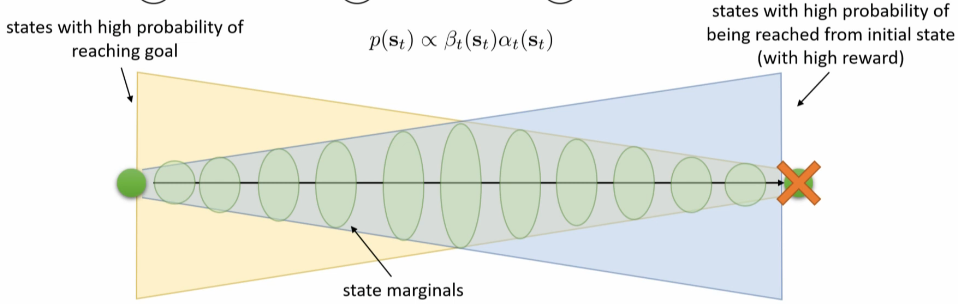
\includegraphics[width=0.8\linewidth]{figures/2020-07-04-202639_958x304_scrot.png}
    \caption{Los \textit{state marginals} es el producto de los mensajes hacia adelante y
    hacia atrás. Normalmente se espera que sean mayores a mitad de la trayectoria. Esto es
consistente con experimentos de comportamiento sobre humanos.}
\end{figure}

\subsection{Resumen}%
\label{sub:resumen}

\begin{itemize}
    \item Se ha introducido un modelo gráfico para hacer control óptimo.
    \item Se ha planteado el control como inferencia (como en HMM, filtros de Kalman, \ldots).
    \item Muy similar a la programación dinámica, iteración de valor, \ldots (pero suave).
\end{itemize}

 \section{¿Hay una explicación mejor?}%
 \label{sec:_hay_una_explicación_mejor_}

 \subsection{El problema del optimismo}%
 \label{sub:el_problema_del_optimismo}
 
 Antes se comentó que el logaritmo de 12.13 es demasiado optimista. Esto es porque se está
 haciendo la pregunta incorrecta. El problema de inferencia es $p(s_{1:T},a_{1:T}|O_{1:T}$,
 marginalizando y condicionando, se obtiene $p(a_t|s_t,O_{1:T})$ (que es la política). Esto es
 el equivalente a preguntar: dado que has obtenido una alta recompensa, ¿cual fue la
 probabilidad de tu acción? Parece una pregunta razonable.

 Pero también se puede marginalizar y condicionar la dinámica,
 $p(s_{t+1}|s_t,a_t,O_{1:T})\neq p(s_{t+1}|s_t,a_t)$. Esto no es igual a la dinámica real del
 entorno, porque es lo mismo que preguntar: dado que has obtenido una recompensa alta,
 ¿cuál fue tu probabilidad de transición? Desde el punto de vista de la inferencia es
 correcto, pero desde el punto de vista del control es curioso, por ejemplo, comprar un ticket de
 lotería porque no se puede planificar ganarla.

 Para arreglar el problema, se quiere resolver la primera pregunta y no la segunda. Esto se
 consigue preguntando: dado que has obtenido una recompensa alta, ¿cuál fue la probabilidad de
 la acción tomada, dado que la probabilidad de transición no cambió? Esta es una pregunta difícil
 de realizar en este problema de inferencia.

 Se tiene que encontrar una distribución $q(s_{1:T},a_{1:T})$ que sea próxima a
 $p(s_{1:T},a_{1:T}|O_{1:T})$ pero que tiene la misma dinámica $p(s_{t+1}|s_t,a_t)$. Este
 problema de encontrar una distribución similar a otra para resolver problemas de
 inferencia en el tema 10.

 Sea $x=O_{1:T}$ y $z=(s_{1:T},a_{1:T})$. Se busca $q(z)$ que aproxime $p(z|x)$. Se va a
 hacer con inferencia variacional. Sea:
 \begin{align}
q ( s _ { 1 : T } , a _ { 1 : T } ) = p ( s _ { 1 } ) \prod _ { t } p ( s _ { t + 1 } | s _ { t } , a _ { t } ) q ( a _ { t } | s _ { t } )
 \end{align}
 Donde se ve que el estado inicial y la dinámica es la misma que en $p$ (haciendo alusión a
 la última parte de la pregunta). $q(a_t|s_t)$ es lo que se va a convertir en la política.

\begin{figure}[H]
	\centering
	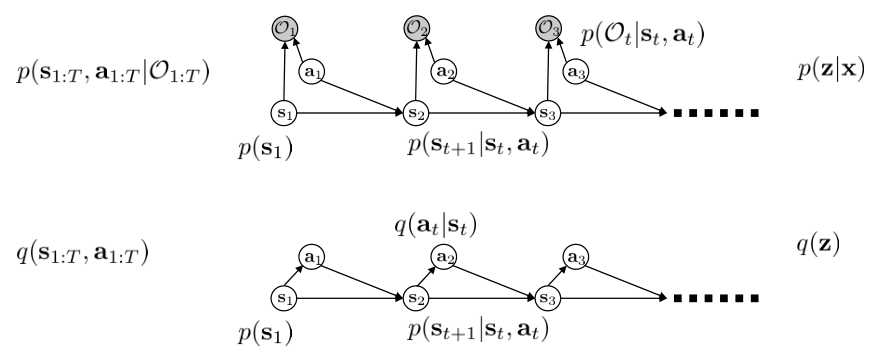
\includegraphics[width=0.8\linewidth]{figures/2020-07-04-205833_888x356_scrot.png}
\end{figure}

Se escribe la cota variacional inferior:
\begin{align}
\operatorname { log } p ( x ) \geq E _ { z \sim q ( z ) } [ \operatorname { log } p ( x , z ) - \operatorname { log } q ( z ) ]
\end{align}
El término de la derecha es $H(q)$ (entropía). Sustituyendo en esta ecuación la $p$ y $q$ que se
han elegido para este problema de control se tiene:
\begin{align}
    \nonumber\operatorname { log } p ( O _ { 1 : T } ) &\geq E _ { ( s _ { 1 : T } , a _ { 1 : T } ) \sim q } [
\operatorname { log } p ( s _ { 1 } ) + \sum _ { t = 1 } ^ { T } \operatorname { log } p ( s _ { t + 1 } | s _ { t } , a _ { t } ) + \sum _ { t = 1 } ^ { T } \operatorname { log } p ( O _ { t } | s _ { t } , a _ { t } )
                                                     \\&\quad\quad\quad\quad\quad\quad - \operatorname { log } p ( s _ { 1 } ) - \sum _ { t = 1 } ^ { T } \operatorname { log } p ( s _ { t + 1 } | s _ { t } , a _ { t } ) - \sum _ { t = 1 } ^ { T } \operatorname { log } q ( a _ { t } | s _ { t } ) ]
\\
  &= E _ { ( s _ { 1 : T } , a _ { 1 : T } ) \sim q } [ \sum _ { t } r ( s _ { t } , a _ { t } ) - \operatorname { log } q ( a _ { t } | s _ { t } ) ]
\end{align}
El resultado se empieza a parecer mucho al objetivo de RL. Se puede sacar el sumatorio fuera de
la esperanza:
\begin{align}
= \sum _ { t } E _ { ( s _ { t } , a _ { t } ) \sim q } [ r ( s _ { t } , a _ { t } ) + H ( q ( a _ { t } | s _ { t } ) ) ]
\end{align}
El objetivo es el mismo que el de RL lo único que se añade la entropía de $q$. Por lo que al
maximizar se está maximizando tanto la recompensa como la entropía.

\begin{algorithm}
    \caption{Paso hacia atrás - variacional}
    \For{$t=T-1$ hasta  $1$}{
        $ Q _ { t } ( s _ { t } , a _ { t } ) = r ( s _ { t } , a _ { t } ) + E [ ( V _ { t + 1 }
        ( s _ { t + 1 } ) ] $\\
        $ V _ { t } ( s _ { t } ) = \operatorname { log } \int \operatorname { exp } ( Q _ { t } ( s _ { t } , a _ { t } ) ) d a _ { t } $
    }
\end{algorithm}

\section{Q-Learning con soft-optimality}%
\label{sec:q_learning_con_soft_optimality}

En el algoritmo estándar de Q-Learning, la actualización de los parámetros se hace como: $ \phi
\leftarrow \phi + \alpha \nabla _ { \phi } Q _ { \phi } ( s , a ) ( r ( s , a ) + \gamma V ( s ^
{ \prime } ) - Q _ { \phi } ( s , a ) ) $ y el objetivo del valor es: $ V ( s ^ { \prime } ) =
\operatorname { max } _ { a ^ { \prime } } Q _ { \phi } ( s ^ { \prime } , a ^ { \prime } ) $.

El único cambio es cambiar el máx por softmax:
\begin{itemize}
    \item Actualización: $ \phi \leftarrow \phi + \alpha \nabla _ { \phi } Q _ { \phi } ( s , a ) ( r ( s , a ) + \gamma V ( s ^ { \prime } ) - Q _ { \phi } ( s , a ) ) $
    \item Objetivo del valor: $ V ( s ^ { \prime } ) = \operatorname { soft } \operatorname { max } _ { a ^ { \prime } } Q _ { \phi } ( s ^ { \prime } , a ^ { \prime } ) = \operatorname { log } \int \operatorname { exp } ( Q _ { \phi } ( s ^ { \prime } , a ^ { \prime } ) ) d a ^ { \prime } $
\end{itemize}
Después de hacer esto, en vez de tener una política voraz se debe de tener una política basada
en el exponente del \textit{advantage}.

\begin{algorithm}
    \caption{Q-Learning with soft-optimality}
    \Repeat{mientras se siga entrenando}{
        Tomar una acción $a_i$ y observar $(s_i,a_i,s'_i,r_i)$, añadirlo a $R$.\\
        Sacar un mini-batch $\{s_j,a_j,s'_j,r_j\}$ de $R$ uniformemente.\\
        Calcular  $ y _ { j } = r _ { j } + \gamma \operatorname { soft } \operatorname { max } _
        { a _ { j } ^ { \prime } } Q _ { \phi ^ { \prime } } ( s _ { j } ^ { \prime } , a _ { j }
        ^ { \prime } ) $ usando la red objetivo $Q_{\phi'}$\\
        $ \phi \leftarrow \phi - \alpha \sum _ { j } \frac { d Q _ { \phi } } { d \phi } ( s _ {
        j } , a _ { j } ) ( Q _ { \phi } ( s _ { j } , a _ { j } ) - y _ { j } ) $\\
        Actualizar $\phi'$: copiar $\phi$ cada $N$ pasos o Polyak
    }
\end{algorithm}

\section{Policy Gradient con soft-optimality}%
\label{sec:policy_gradient_con_soft_optimality}

\begin{align}
\pi ( a | s ) = \operatorname { exp } ( Q _ { \phi } ( s , a ) - V ( s ) ) \text { optimiza } \sum _ { t } E _ { \pi ( s _ { t } , a _ { t } ) } [ r ( s _ { t } , a _ { t } ) ] + E _ { \pi ( s _ { t } ) } [ H ( \pi ( a _ { t } | s _ { t } ) ) ]
\end{align}

Intuición:
\begin{align}
\pi ( a | s ) \propto \operatorname { exp } ( Q _ { \phi } ( s , a ) ) \text { cuando } \pi
\operatorname { minimiza } D _ { KL } ( \pi ( a | s ) \| \frac { 1 } { Z } \operatorname { exp }
( Q ( s , a ) ) )\\
D _ { KL } ( \pi ( a | s ) \| \frac { 1 } { Z } \operatorname { exp } ( Q ( s , a ) ) ) = E _ { \pi ( a | s ) } [ Q ( s , a ) ] - H ( \pi )
\end{align}

Normalmente se le llama Entropy Regularized Policy Gradient. Combate contra el colapso de la
entropía de Policy Gradient normal, lo que lleva a que la varianza se reduzca mucho al
principio y reduzca la exploración.

Esta modificación se utilizaba de forma heurística antes de averiguar el porque.

Está muy relacionado con soft Q-Learning (Haarnoja et al. 2017 y Schulman et al. 2017).

\section{Beneficios de la optimalidad blanda}%
\label{sec:beneficios_de_la_optimalidad_blanda}

\begin{itemize}
    \item Mejora la exploración y previene los colapsos de entropía
    \item Es más fácil ajustar políticas más finamente a tareas más específicas
    \item Rompe los empates de acciones con igual probabilidad
    \item Más robusto debido a que se ven más estados (porque se maximiza la entropía).
    \item Se puede reducir a optimalidad dura según la mangitud de la recompensa vaya
        incrementándose.
\end{itemize}
